% Carsten: Once more, the reasons for reading this chapter must be stated clearly at the
% start of this chapter, and it must be founded on section 1.3, or perhaps be a
% consequence of knowledge found in chapter 2, which leads to the assumption that gestures are a desirable approach to interaction. 
% If it is a consequence, than the motivation for looking deeper into gestures should be included in the conclusion of chapter 2.
This chapter will review what gesture recognition is, what technology that enables it, and how it can potentially give new possibilities when working
with three-dimension environments, like our design review application will. Furthermore, using gesture recognition technology with virtual reality is 
of special interest as virtual reality in many ways change several human-computer interaction patterns. This chapter will also compare several competing 
technologies that enable gesture recognition, and use this comparison as a foundation for the design and implementation of the design review application.  

\section{Gestures}
According to research, non-verbal communication makes up about two-thirds of all communication between humans, with gestures being one of the most common 
categories of non-verbal communication, often conveying the most specific linguistic content~\citep{Hogan2003}.
A gesture can be defined as a physical movement of the hands, arms, face and body with the intent to convey information or meaning~\citep{Mitra2007}, 
and can often be classified into several categories, some of which are mention in section~\vref{sec:gesture_classes}. Even though 
a gesture can involve several body parts hand gestures are of special interest to this thesis, as they are often the most used in non-verbal communication
and the most convenient to utilize in our design review application. 
Gesture as an interaction and communication method not only between humans, but also between human and computer is an interesting topic, 
and especially so when it comes to virtual reality as it sets some constraints with regard to more conventional interaction methods, like using 
a mouse and keyboard. \citet{Rautaray2015} also points out that there are situations in which
these devices are impractical for human-computer interaction (HCI), and that this is particularly the case for interaction with 3D objects.
As mentioned earlier, gestures can be divides into several categories, with two of the primary ones being \textit{static gestures} and \textit{dynamic gestures}.

\subsection{Static and Dynamic Gestures}
\label{sec:gesture_classes}
In the gesture recognition field it is common to define a gesture as either a static or dynamic. Static gestures can in simple terms be defined as gestures
without any movement. The hand and its fingers and joints simply maintain a certain position or orientation and it is recognized as a gesture. One example 
of this gesture category is the "V sign" (or the "peace sign"), where the index and middle fingers are raised and parted while the other fingers are clenched.

Dynamic gestures, on the other hand, are gesture that involves or requires movement for the gesture to have semantic meaning. One example of this
might be to wave goodbye to someone or to twist a straight hand back and forth to indicate uncertainty. One can classify dynamic gestures into several 
subclasses, such as conscious gestures, which are done intentionally for communication purposes, or unconscious gestures, which are carried out unconsciously.
See~\vref{fig:static_and_dynamic} for an hierarchical overview.
%As the gestures included in this thesis' implementation can be considered static (they use movement, but does not require it)

\begin{figure}%[h!] %[H]
	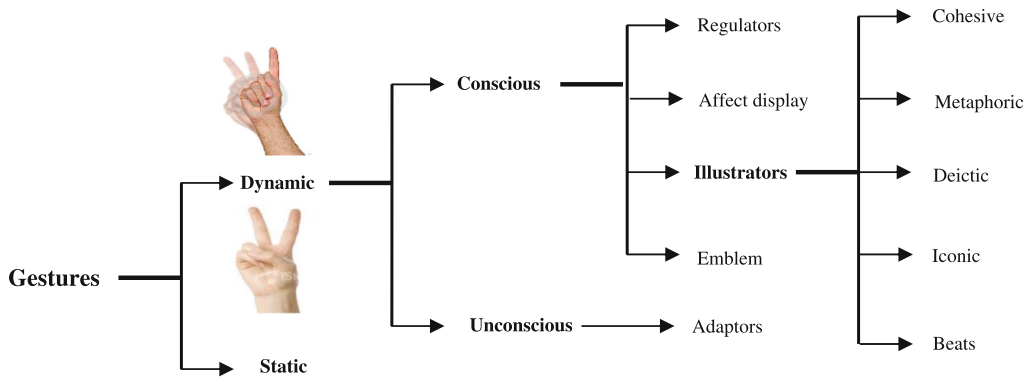
\includegraphics[width=\linewidth]{pictures/static_and_dynamic.png}
	\caption[The vision-based hand gesture categories]{The vision-based hand gesture categories~\citep{Kanniche2009}.}
	\label{fig:static_and_dynamic}
\end{figure} 


What gesture types are being used has implication for the gesture recognition methods as well. 

\section{Gesture Recognition Devices}
\label{sec:gr_devices}
\import{}{gr_devices.tex}


\section{The Vision-based Recognition Pipeline}
\label{sec:gr_principles}
\import{}{gr_principles.tex}



% Carsten: Conclude the chapter with insights gained for the thesis, and consequences for your work on the thesis, such as choices made and work you have to do. 
% In this particular case, the conclusion must also create a smooth transition to chapter 4, because it’s focussing more on a special case 
% of the things that you’ve just introduced.
% Provide already in the conclusion of 3 a hint why there is so much to tell about the Leap Motion that it’s worth its own chapter.